\documentclass[11pt, a4paper]{article}
\usepackage{amsmath, amsthm, amssymb, calrsfs, wasysym, verbatim, bbm, color, graphics, geometry}
\usepackage[utf8]{inputenc} % comment when using lualatex
%\usepackage[italian]{babel} % lingua e a-capo-sillabato
\usepackage{fullpage}
\usepackage{graphicx}
%\usepackage[hidelinks]{hyperref,xcolor} % link di pagina
\usepackage[bottom]{footmisc} % note appiccicate al fondo della pagina
\usepackage{float} % per posizionamento immagini
\usepackage{cancel}
\usepackage{tikz}
\usepackage{framed}
\usepackage{amsfonts}

\geometry{tmargin=.75in, bmargin=.75in, lmargin=.75in, rmargin = .75in}  

\newcommand{\R}{\mathbb{R}}
\newcommand{\C}{\mathbb{C}}
\newcommand{\Z}{\mathbb{Z}}
\newcommand{\N}{\mathbb{N}}
\newcommand{\Q}{\mathbb{Q}}
\newcommand{\M}{\mathbb{M}}
\newcommand{\enc}{\mathcal{E}nc}
\newcommand{\dec}{\mathcal{D}ec}
\newcommand{\negl}{\text{negl}}
\newcommand{\poly}{\text{poly}}
\newcommand{\game}{\text{GAME}}
\newcommand{\Cdot}{\boldsymbol{\cdot}}

\newtheorem{thm}{Theorem}
\newtheorem{defn}{Definition}
\newtheorem{conv}{Convention}
\newtheorem{rem}{Remark}
\newtheorem{lem}{Lemma}
\newtheorem{cor}{Corollary}



\definecolor{dkgreen}{rgb}{0,0.6,0}
\definecolor{gray}{rgb}{0.5,0.5,0.5}
\definecolor{mauve}{rgb}{0.58,0,0.82}


\title{Cryptography Notes }
\author{Raffaele Castagna}

\date{Academic Year 2025-2026}

\begin{document}

\maketitle
\tableofcontents
\newpage

\section{Intro to Cryptography}
\label{Intro}
\subsection{Secure Communication}
We have multiple goals in cryptography, the most important ones being:
\begin{center}
    \textbf{Confidential Integrity}
    \includegraphics{img/CF comm.png}
\end{center}
\begin{center}
    \textbf{Message Integrity}
    \includegraphics{img/Msg int.png}
\end{center}
Basically we want our message to be both \textbf{confidential}, so no-one except the intended target sees it and we it to be unmodified, so that its \textbf{integrity} has not been compromised.\\\\
There are many different ways to do this, but in our case we only see two major ways:
\begin{itemize}
    \item \textbf{Symmetric Cryptography}:  $\text{Where Alice and Bob share a key } k \in \mathcal{K} \text{,the key is random and unknown to Eve}$
    \item \textbf{Assymetric Cryptography}: Where Alice and Bob do not share a key, but they have each their own key pair $(p_k,s_k)$ where $p_k$ is the public key and $s_k$ is the secret/private key
\end{itemize}

\subsection{Unconditional Security}
To achieve confidential communication, we use symmetric cryptography.
\begin{center}
    \includegraphics{img/US.png}
\end{center}
With $m \in \mathcal{M}, c \in \mathcal{C}, k \in \mathcal{K}$\\\\
In this case we have Alice sending a message \textit{m} which is then encrypted utilizing a randomly generate key \textit{k} to generate the cyphertext \textit{c}, after that to get back to the initial message \textit{m}, Bob will then need to decrypt it utilizing his own key \textit{k} on cyphertext \textit{c}.\\
In a more formal way we can define Symmetric encryption (SKE) as $\prod = (Enc, Dec)$ such that:
\begin{itemize}
    \item Enc : $\mathcal{M} \times \mathcal{K} \rightarrow \mathcal{C}$
    \item Dec: $\mathcal{C} \times \mathcal{K} \rightarrow \mathcal{C}$
    \item k is uniform over $\mathcal{K}$ (k is chosen according to some distribution)
\end{itemize}
An encryption scheme must satisfy the correctness requirement:
\begin{defn}
    $\forall k \in \mathcal{K}, \forall m \in \mathcal{M} \text{ it holds that } Dec(k,Enc(k,m)) = m$
\end{defn}

\textbf{Kerchoff's Principle}:
\begin{defn}
    Security should not depend on the secrecy of the algorithm but on the secrecy of the key.
\end{defn}
\subsection{Perfect Secrecy}
\begin{defn}
Let M be any distribution over $\mathcal{M}$ and K be uniform over $\mathcal{K}$ (Then observe C = Enc(K,M) in a distribution over C), we say that (Enc,Dec) = $\prod$ is \textbf{perfectly secret}
if $\forall M, \forall m \in \mathcal{M}, \forall c \in \mathcal{C}: Pr[M=m] = Pr(M=m | C=c)$ (The probability that M is m is equal to the probability that M is m knowing that C is c, so by knowing the cyphertext, we dont gain additional information).
\begin{lem}
The following are equivalent:
\begin{itemize}
    \item Perfect Secrecy
    \item M and C are independant
    \item $\forall m,m' \in \mathcal{M}, \forall c \in \mathcal{C}: Pr[Enc(k,m) = c] = Pr[Enc(k,m') = c] \text{ with k being uniform over } \mathcal{K}$
\end{itemize}
\end{lem}
\end{defn}
\subsection{OTP}
Let us see if OTP (\textit{One Time Pad}) is perfectly secret\\
We know that the OTP uses $\oplus$ to generate and later decypher the cyphertext, we have that $K=M=C=\{0,1\}^N$ with N being the length of the string, we know that:
\begin{itemize}
    \item Enc (k,m) = $k \oplus m$
    \item Dec (k,c) = $c \oplus k$ = $(k \oplus m) \oplus k = m$
\end{itemize}
To prove that it is perfectly secret let us utilize the third lemma:
\begin{center}
    $Pr[C=c | M=m'] = Pr[\text{Enc}_k (m') = c] = Pr[m' \oplus K = c] = Pr[K = m' \oplus c] = 2^{-N}$
\end{center}
and therefore:\\
\begin{center}
    $Pr[Enc(k,m') = c] = 2^{-N}$
\end{center}
There seem to be some limitations, the key can only be used once and it must as long as the message,lets assume we encrypt m'' and m':
$c_1 = k \oplus m_1\text{    } c_2 = k \oplus m_2 \text{ therefore } c_1 \oplus c_2 = m_1 \oplus m_2$, so if I know a pair $(m_1,c_1) \text{ then I could compute } m_2$, therefore we cannot encrypt two messages with the same key.
\begin{thm}[Shannon]
Let $\prod$ be any perfectly secret SKE then we have $|\mathcal{K}| \ge |\mathcal{M}|$.
\end{thm}
\begin{proof}
Take $\prod$ to be uniform over $\mathcal{M}$. Take any c s.t. Pr[C=c] $>$ 0.\\
Consider $\mathcal{M'} = \{Dec(k,c): k \in \mathcal{K}\}$ and assume $|\mathcal{K}| < |\mathcal{M}|$ by contraddiction, then:\\
\begin{center}
    $|\mathcal{M}|' \leq |\mathcal{K}| < |\mathcal{M}| \rightarrow |\mathcal{M'}| < |\mathcal{M}| \rightarrow \exists m \in \mathcal{M} \setminus \mathcal{M'}$
\end{center}
Now:\\
\begin{center}
   $ Pr[M=m] = |\mathcal{M}|^{-1} \text{ but } Pr[M=m | C=c] = 0 $
\end{center}

\end{proof}

\subsection{Proof that the lemmas imply eachother}
Let us prove that $1 \implies 2 \implies 3 \implies 1$\\\\
Let us start by proving that $1\implies2$:
\begin{proof}
We know that $Pr[M=m] = Pr[M=m|C=c] \rightarrow \frac{Pr[M=m \wedge C=c]}{Pr[C=c]} = Pr[M=m \wedge C=c] \\= Pr[M=m] * Pr[C = c]$
and therefore we have proved their independence, so $I(M;C) = 0$
\end{proof}
Let us prove that $2 \implies 3$
\begin{proof}
Let us fix an m from M and c from C:\\
$Pr[Enc(K,m) = c] = Pr[Enc(K,M) = c | M = m] \implies Pr[C = c | M = m] = Pr[C=c]$ \\Remember that Enc(...) is c!\\\\ We do the same thing for $m'$ and we get: 
$Pr[C=c | M=m] = Pr[C=c]$ for both of them.\\
Therefore: $Pr[Enc(K,m')= c] = Pr[C=c]$
\end{proof}

And now $3 \implies 1$:
Take any c from C:\\
$Pr[C=c] = Pr[C=c|M=m]$ by 2 (we are claiming this)\\\\
If the claim is true then:\\
$Pr[M=m|C=c] * Pr[C=c] = Pr[M=m \wedge C=c] = Pr[C = c | M = m] * Pr[M=m] \implies$\\\\
\begin{center}
   $\implies$ $Pr[M=m] = \frac{Pr[M=m | C=c] * \cancel{Pr[C=c]}}{\cancel{Pr[C=c|M=m]}}$

\end{center}
However we still need to prove the claim:\\
$$Pr[C=c] = \sum_{m'}^{}Pr[C=c \wedge M=m'] = \sum_{m'}^{}Pr[C=c | M=m'] * Pr[M=m'] =$$\\ $$\sum_{m'}^{}Pr[Enc(K,m') = c | M=m'] * Pr[M=m']\\= \sum_{m'}^{}Pr[Enc(K,m') = c] * Pr[M=m'] $$\\
$$ \sum_{m'}^{}Pr[Enc(k,m) = c] * Pr[M=m'] = Pr[Enc(k,m) = c] * \sum_{m'}^{}Pr[M=m'] \impliedby 1$$\\
$$ Pr[Enc(k,m) = c] = Pr[Enc(K,M) = c | M=m] \rightarrow Pr[C=c | M=m]$$
\subsection{Message Authentication Codes}
\begin{center}
    \includegraphics[scale=0.5]{img/MAC.png}
\end{center}
In case it is $\tau$ then we accept it, else no.\\
There is no need to prove correctness as $\tau$ is deterministic, so if we had the same k and m, we should get the same $\tau$\\\\
\textbf{Unforgeability}\\\\
It should be hard to forge $\tau'$ such on msg m' and it should be hard to produce (m,$\tau$) as long as m' $\neq$ m\\
\begin{defn}
\textbf{Statistical secure MAC} We say that $\prod$ = Tag has $\epsilon$-statistical security (unforgeability) if  $\text{ }\forall m,m'\text{ } \in \mathcal{M} \text{ with } m \neq m'\text{ } \forall \tau,\tau' \in \mathcal{T}$:\\
$$Pr[Tag(K,m') = \tau'\text{ } | \text{ }Tag(K,m)= \tau] \leq \epsilon$$
\end{defn}
\textbf{TLDR}: Fix \underline{any} m,m' with m' $\neq$ m take $\tau,\tau'$ on the condition that $\tau$ is tag of m and given $\tau'$, it is always less than or equal to $\epsilon$\\
Here $\epsilon$ is a parameter e.g. $2^{-80}$\\
\textbf{Exercise} Let us prove that it is impossible to get $\epsilon = 0$\\
Because a random $\tau' \in \mathcal{T}$ has probability $\geq \frac{1}{|\mathcal{T}|}$ to be correct it is impossible.\\\\
Note that the definition is valid for One-Time!\\
We will show:
\begin{itemize}
    \item The notion is Achievable
    \item It's inefficient, in fact:
\end{itemize}
\begin{thm}
    Any t-time $2^{-\lambda}$ statistically secure Tag has a key of some (t+1)*$\lambda$
\end{thm}
We will now show that any form of hash function with a particular property satisfies the definition.\\
\begin{defn}
    \textbf{Pairwise independence} A family $\mathcal{H} = \{h_k: \mathcal{M} \rightarrow \mathcal{T}\}_{k \in \mathcal{K}}$ is pairwise independant if: $\forall m,m' \in \mathcal{M} \text{s.t.} m \neq m'$ then:
    $(h(K,m),h(K,m'))$ is uniform over $\mathcal{T}^2 = \mathcal{T} \times \mathcal{T}$ for K uniform over $\mathcal{K}$
\end{defn}

\begin{thm}
    Any family $\mathcal{H}$ of pairwise independent functions directly gives a $\epsilon = \frac{1}{|\mathcal{T}|}-\text{statistically}$ secure MAC.
\end{thm}
\begin{proof}
    Fix any $m \in \mathcal{M}, \tau \in \mathcal{T}$:\\
    $$Pr[Tag(K,m) = \tau] =$$ \\$$ Pr_k[h(K,m)= \tau] = \frac{1}{|\mathcal{T}|}\text{ by pairwise independence}$$\\
    Similiarly, for any m,m' s.t. m $\neq$ m', $\tau,\tau' \in \mathcal{T}$.
    $$Pr_k[Tag(K,m)= \tau \wedge Tag(K,m') = \tau'] =$$
    $$Pr_k[h(K,m)=\tau \wedge h(K,m')= \tau'] = \frac{1}{|\mathcal{T}|^2}$$
    By Bayes:
    $$Pr[Tag(K,m')= \tau' | Tag(K,m) = \tau] = $$
    $$\frac{Pr[h(K,m;) = \tau' \wedge h(K,m) = \tau]}{Pr[h(K,m) = \tau]} =$$
    $$\frac{\frac{1}{|\mathcal{T}|^2}}{\frac{1}{|\mathcal{T}|}} = \frac{1}{|\mathcal{T}|}$$

\end{proof}
Now we need to instantiate it, here is a construction, Let p be a prime:\\
    $$h_{a,b}(m) = am+b \mod p $$
    $$k = (a,b) \in \Z_{p}^2 = \mathcal{K}$$
    $$\Z_p = \mathcal{M} =\mathcal{T}$$
\begin{lem}
    The above $\mathcal{H}$ is \textit{pairwise independant}.
\end{lem}
\begin{proof}
    For all $m,m' \in \Z_p , \tau,\tau' \in \Z_p$ with $m \neq m'$\\
    $$\Pr_{(a,b) \in \Z_{p}^2}[h_{a,b}(m) = \tau \wedge h_{a,b}(m') = \tau'] =$$
    $$\Pr_{(a,b) \in \Z_{p}^2}\left[
        \begin{pmatrix}
        m & 1 \\ m' & 1
        \end{pmatrix}
        \begin{pmatrix}
            a \\ b
        \end{pmatrix} =
        \begin{matrix}
            \tau \\ \tau'
        \end{matrix}\right] = $$ 
        $$\Pr_{(a,b) \in \Z_{p}^2}\left[
        \begin{pmatrix}
            a \\ b
        \end{pmatrix} =
        \begin{pmatrix}
        m & 1 \\ m' & 1
        \end{pmatrix}
        \begin{matrix}
            \tau \\ \tau'
        \end{matrix}\right] = $$
        $$\frac{1}{p^2} = \frac{1}{|\Z_{p}|^2} = \frac{1}{|\mathcal{T}|^2}$$
\end{proof}
\subsection{Randomness Extraction}
Alice and Bob need a \textbf{random} key, how can they generate it?\\
Randomness is crucial for crypto, and two components are necessary in any RNG (e.g. Fortuna, /dev/rand):\\
\begin{itemize}
    \item Randomness extraction: By measuring physical quantities we can get an \textbf{unpredictable} sequence of bits (Not necessarily uniform or for cheap!)\\ From this we extract a \textbf{random} Y which is short (e.g. 256 bits)
    \item Expand it to any amount (polynomial) using a psedorandom generator (PRG) - but this requires computational assumptions.
\end{itemize}
We want to understand how to extract from an unpredictable source X.\\
\textbf{Example \textit{Von Neumann Extractor}}
Assume $B \in {0,1} \text{ s.t. } \Pr[B=0] = p < \frac{1}{2}$.
\begin{itemize}
    \item Sample $b_1 \in B, b_2 \in B$
    \item if $b_1 = b_2$ then Resample
    \item Else output 1 $\iff b_1 = 0, b_2 = 1, \text{ or 0 if } b_1 = 1, b_2 =0$
\end{itemize}
Assuming it outputs something, this will be s.t.\\
$$\Pr[\text{Output 0}] = Pr[\text{Output 1}] = p*(1-p)$$
$$\Pr[\text{No output after N tries}] = (1-2p(1-p))^N \text{ which becomes small for large enough N}$$
We want to generalize this question, ideally we want to design a function Ext that takes a random variable X and outputs an uniform Ext(X), but this is impossible as the source must be unpredictable and Ext is deterministic
\begin{defn}[Min-Entropy]
    The min-entropy of X is: $H_{\infty} = - \log_2\max{\Pr[X=x]}$
\end{defn}
\textbf{Example}:
Let $X \equiv U_m$ Uniform over $\{0,1\}^{N}$. $ H_{\infty} (X) = N$\\
If X is a costant we have $H_\infty (X)$ = 0
\\\\
Here's the next best thing:\\
Design Ext that extracts UNIFORM $Y=Ext(X)$ for every X s.t. $H_\infty (X) \geq k$\\
But this is also impossible, even if $$Ext(X)= b \in \{0,1\}$$ $$k = n-1$$ $$x \in \{0,1\}^n$$\\
And here's why: fix any Ext:$\{0,1\}^n \rightarrow {0,1}$ and let $b \in {0,1}$ be the output of maximing $|Ext^{-1}(b)|$\\
\begin{center}
    \includegraphics[scale=0.3]{img/expl.png}
\end{center}
The bad X: Define X to be Uniform over $Ext^{-1}(b)$. Since it is uniform: $H_\infty(X) \geq n-1$ but $Ext(X) = b$ so not uniform.\\\\
Solution: Swap the quantifiers.
\begin{defn}[Seeded Extractor]
    A function $Ext: \{0,1\}^n \times \{0,1\}^d \rightarrow \{0,1\}$ is a (k,$\epsilon$)-seeded extractor if for every X over s.t. $H_\infty(X) \geq k$: $$(S,Ext(S,X)) \approx_\epsilon (S,U_e)$$
    for $S \equiv U_d$ (uniform over $\{0,1\}^d$). (Note that $(S,U_e) \equiv U_{d+e}$).
\end{defn}
What does this mean? There is a standard way to measure distance between distributions:
$$ Z \equiv_\epsilon Z' \iff SD(Z,Z') \leq \epsilon$$
$$ SD(Z,Z') = \frac{1}{2} \sum_{z} |Pr[Z=z] - Pr[Z'=z]|$$
This is equivalent: $\forall$ Unbounded adversary A:
$$|Pr[A(z)=1 : z \in Z] - Pr[A(z)=1 : z \in Z']| \leq \epsilon$$
\begin{thm}[Leftover Hash Lemma]
    Let $\mathcal{H} = \{h_s: \{0,1\}^n \rightarrow \{0,1\}^l\}_{s \in \{0,1\}^d}$ be a family of pairwise independent hash functions. Then Ext(x,s) = $h_s(x)$ is a (k,$\epsilon$)-seeded extractor for k $\geq l + 2\log_2(\frac{1}{\epsilon})$-2.

\end{thm}
\begin{lem}
    Let Y be a RV over $\mathcal{Y}$. Such that:
    $$Col(Y) = \sum_{y \in \mathcal{Y}} Pr[Y=y]^2 \leq \frac{1}{|\mathcal{Y}|} * (1 + 4\epsilon^2)$$
    Then, SD(Y,U) $\leq \epsilon$
\end{lem}
\begin{proof}
    $$SD(Y,U) = \frac{1}{2} \sum_{y \in \mathcal{Y}} |Pr[Y=y] - \Pr[U=y]|$$
    $$\frac{1}{2} \sum_{y \in \mathcal{Y}} |Pr[Y=y] - \frac{1}{|\mathcal{Y}|}|$$
    $$\text{Let } q_y = Pr[Y=y] - \frac{1}{|\mathcal{Y}|}$$
    $$\text{Let } s_y = \begin{cases}
        1 \text{ if } q_y \geq 0\\
        -1 \text{ else}
    \end{cases}$$
    $$\text{Hence } SD(Y,U) = \frac{1}{2} \sum_{y \in \mathcal{Y}} s_y q_y$$
    $$= \frac{1}{2} \langle s,q \rangle \leq \frac{1}{2} \sqrt{<\overrightarrow{q},\overrightarrow{q}> * <\overrightarrow{s},\overrightarrow{s}>} \text{ by Cauchy-Schwarz}$$
    $$ = \frac{1}{2} \sqrt{\sum_{y \in \mathcal{Y}} q_y^2 * |\mathcal{Y}|}$$

Now, We analyze the term $\sum_{y \in \mathcal{Y}} q_y^2$:
$$\sum_{y \in \mathcal{Y}} q_y^2 = \sum_{y \in \mathcal{Y}} (Pr[Y=y] - \frac{1}{|\mathcal{Y}|})^2 =$$
$$\sum_{y \in \mathcal{Y}} Pr[Y=y]^2 + \frac{1}{|\mathcal{Y}|^2} -2\frac{Pr[Y=y]}{|\mathcal{Y}|} =$$
$$ \underbrace{\sum_{y \in \mathcal{Y}} \Pr[Y=y]^2}_{Col(Y)} + \frac{1}{|\mathcal{Y}|} - 2\frac{1}{|\mathcal{Y}|} =$$
$$Col(Y) - \frac{1}{|\mathcal{Y}|} \leq \frac{4\epsilon^2}{|\mathcal{Y}|}$$
Then:
$$SD(Y,U) \leq \frac{1}{2} \sqrt{\frac{4\epsilon^2}{\cancel{|\mathcal{Y}|}} * \cancel{|\mathcal{Y}|}} = \epsilon$$
\end{proof}
Next we apply the lemma to prove the Leftover Hash Lemma:
\begin{proof}
    $$Y = (S,Ext(X,S)) = (S,h(S,X))$$
and compute Col(Y):
$$Col(Y) = \sum_{y \in \mathcal{Y}}\Pr[Y=y]^2 = \Pr[Y=Y']$$
$$= \Pr[S=S' \wedge h(S,X) = h(S',X')]$$
$$= \Pr[S=S' \wedge h(S,X) = h(S,X')]$$
$$= \Pr[S=S'] * \Pr[h(S,X) = h(S,X')]$$
$$= \frac{1}{2^d} * \Pr[h(S,X) = h(S,X')]$$
$$ = \frac{1}{2^d} * (\Pr[X=X'] + \Pr[h(S,X) = h(S,X') \wedge X \neq X'])$$
$$ \leq \frac{1}{2^d} * (\frac{1}{2^k} + \frac{1}{2^l}) \text{ by pairwise independence and } H_\infty(X) \geq k$$
$$ = \frac{1}{2^{d+l}}(1 + 2^{l-k}) \leq \frac{1}{2^{d+l}}(2^{2-2\log_2(\frac{1}{\epsilon})}+ 1)$$
$$ = \frac{1}{|\mathcal{Y}|} * (1 + 4\epsilon^2)$$ 
\end{proof}
\section{Computational Security}
We know that withouth any assumptions we can do Symmetric crypto and randomness generation, with some strong limitations.\\
\begin{itemize}
    \item Privacy: $|msg| = |key|$ and one-time use
    \item Integrity: same as above.
    \item Randomness We can't extract more than k from $p_y k$
\end{itemize}
We want to overcome all these limitations. We'll do so off of the base of some assumptions
\begin{itemize}
    \item Adversary is Computationally Bounded
    \item Hard Problems exist
\end{itemize}
We will make conditional statements:
\begin{thm}
    If Problem X is hard (against efficient solvers), Then cryptosystem $\prod$ is secure (against efficient adversaries)
\end{thm}
Consequence: if $\prod$ is insecure, $\exists$ efficient solver for X!\\
Depending on what X is, the above could be \textbf{Groundbreaking}.\\\\
\textbf{Examples}:\\
X = $"P \neq NP"$
X = "Factoring is hard"\\
X = "Discrete Log is hard"\\\\
We are not able to just assume $P \neq NP$, we need a stronger assumption:
\textbf{One-Way Functions}: These are functions that are easy to compute but hard to invert.\\
Clearly OWF$ \implies P \neq NP$, why?\\
Because if $P=NP$, OWF do not exist as checking if f(x) = y is efficient and this it's in NP=P\\
We cannot exclude that $P \neq NP$ but still,OWF do not exist.\\\\
To better demonstrate this, we can refer to the following worlds created by Russel Impagliazzo:
\begin{itemize}
    \item Algorithmica: P=NP
    \item Heuristica: P $\neq$ NP but no "average-hard" problems
    \item Pessiland: $P\neq NP$ and "average-hard" problems exist, but no OWF
    \item Minicrypt: OWFs exist
    \item Cryptomania: OWF exist + Public-key crypto exist
\end{itemize}
First we must start by fixing a model of computation: Turing Machines\\
efficient computation = polynomial time TMs.\\
Let's be generous: Adversaries can use any amount (polynomial) of randomness: Probabilistic Polynomial Time (PPT) TMs.\\
In what comes next we could define two approaches:
\begin{itemize}
    \item \textbf{Concrete Security} Security hols w.r.t. t-time Tms except w.p. $\leq \epsilon$ (e.g.  $t= 2^20$ steps, $\epsilon = 2^{-80}$)
    \item \textbf{Asymptotic Security} Let $\lambda$ be a security parameter. Adversaries are poly($\lambda$)-time PPT TMs ($\epsilon$ = negligeble $=$ negl($\lambda$))\\
\end{itemize}
\begin{defn}[Negligible]
    $\epsilon: \N \rightarrow \R$ is negligible if $\forall p(\lambda)=\text{poly}(\lambda) \text{ } \exists \lambda_0 \in \N \text{ s.t. } \forall \lambda > \lambda_0: \epsilon(\lambda) \leq \frac{1}{p(\lambda)}$
\end{defn}
(In other words, $\epsilon(\lambda) \leq O(\frac{1}{p(\lambda)}) \text{  }\forall p(\lambda) = \text{poly}(\lambda))$\\
\subsection{Pseudorandomness}
This is our first step towards efficient symmetric crypto. Moreover, pseudorandomness is used in modern computers to simulate real randomness. We will see that OWF are enough for pseudorandomness.\\
\begin{defn}[OWF]
    A function $f :\{0,1\}^n \rightarrow \{0,1\}^n$ is One-Way, if: $\forall PPT \mathcal{A}$:
    $$\Pr_{x \leftarrow\{0,1\}^n}[f(x')= y : y = f(x); x' \leftarrow \mathcal{A}(y)] \leq \text{negl}(n)$$
\end{defn}
Informally, it goes to zero faster than any inverse of a polynomial function.\\\\
Example of negl(n) is $2^{-n}$\\
An alternative way to think about it:
\begin{center}
    \includegraphics[scale=0.4]{img/Comp_sec/Alternative1.png}
\end{center}
\begin{defn}[Pseudorandomness]
    Pseudorandomness is a sequence of bits that are not random, but look random. We capture this requirement using \textbf{Indistinguishability (computational)}.\\
    We have already seen something like this in SD. Given X,X' RVs over some domain, SD(X,X') $\leq \epsilon$ is equivalent to: $\forall \mathcal{D}$ (adversary):
    $$|Pr[\mathcal{D}(x)=1 : x \leftarrow X] - Pr[\mathcal{D}(y)=1 : y \leftarrow X']| \leq \epsilon$$ 
\end{defn}
\begin{center}
    \includegraphics[scale=0.4]{img/Comp_sec/Alt2.png}
\end{center}
\begin{defn}
    X ($X_n$),Y ($Y_n$) are computationally indistinguishable ($ X \approx_c Y$) if $\forall PPT \mathcal{D}$:
    $$|Pr[\mathcal{D}(z)=1 : z \leftarrow X_n] - Pr[\mathcal{D}(z)=1 : x' \leftarrow Y_n]| \leq \text{negl}(n)$$
\end{defn}
With this we can define pseudorandomness:
\begin{defn}[Pseudorandom Generator (PRG)]
    A function $G: \{0,1\}^n \rightarrow \{0,1\}^{n+l}$ with $l \geq 1$ (The Stretch) is secure if:
    $$G(U_n) \approx_c U_{n+l}$$
    $$U_n \equiv \text{ uniform over } \{0,1\}^n$$
    $$U_{n+l} \equiv \text{ uniform over } \{0,1\}^{n+l}$$
\end{defn}
\begin{center}
    \includegraphics[scale=0.4]{img/Comp_sec/pseudogen.png}
\end{center}
Let's understand how to build PRGs:
\begin{itemize}
    \item Use a randomness extractor to get a uniform seed $s \in \{0,,1\}^n$.
    \item Define a simple PRG $G:\{0,1\}^n \rightarrow \{0,1\}^{n+1}$ with minimal stretch $l = 1$.
    \item Use G to stretch any $l(n) = poly(n)$.
\end{itemize}
Theory vs Practice:
\begin{itemize}
    \item Randomness extraction is what we already studied. But in practice it is done using Hash Functions.
    \item Theoretical G can be obtained from any OWF. Practical G is Heuristic
    \item Stretch is the same
    \item In practice the seed is refreshed periodically collecting new entropy
\end{itemize}
\begin{thm}
    If there exists a PRG $G: \{0,1\}^n \rightarrow \{0,1\}^{n+1},\text{ then there exists a PRG } G^l : \{0,1\}^n \rightarrow \{0,1\}^{n+l} \text{ for any } l(n)=poly(n) $
\end{thm}
\begin{center}
    \includegraphics[scale=0.4]{img/Comp_sec/BlueGen.png}
\end{center}
\begin{proof}
    Assume $G^l$ not secure, $\exists$ PPT $\mathcal{D}^l$ that can distinguish $G^l(U_n)$ from $U_{n+l}$ with probability $\geq \frac{1}{p(n)}$ for some polynomial. We want to buildt PPT $\mathcal{D}$ that can
    distinguish $G(U_n)$ from $U_{n+1}$ with probability $\frac{1}{p(n)}$. ($\mathcal{D}$ is called a reduction)
    \begin{center}
        \includegraphics[scale=0.4]{img/Comp_sec/Hybrid_arg_img.png}
    \end{center}
\section*{Hybrid argument}

\[
H_0(n) \equiv G^{n}(U_m)
\]

\[
b_1, \ldots, b_\ell \leftarrow \{0,1\}^\ell
\]

\[
H_i(M) \equiv
\begin{cases}
b_1, \ldots, b_i \leftarrow \{0,1\} \\
s_i \leftarrow \{0,1\}^n \\
(b_{i+1}, \ldots, b_\ell, s_\ell) = G(s_i)
\end{cases}
\]

\[
H_\ell(n) \equiv U_{\ell + m}
\]

\end{proof}

\begin{lem}
    $\forall i : H_i \approx_c H_{i+1}$.
\end{lem}
\begin{proof}
    By reduction (as before):
    \begin{center}
        \includegraphics[scale=0.4]{img/Comp_sec/Reduction.png}
    \end{center}
    By the above observations:
    $$\Pr[\mathcal{D}(z) = 1: z = G(s); s \in \{0,1\}^n] $$
    $$= \Pr[\mathcal{D}'(b1,\dots,b_\ell,s_\ell) = 1 : (b1,\dots,b_\ell,s_\ell) \in H_i (n)]$$
    $$ \Pr[\mathcal{D}(z) = 1 : z \leftarrow U_{n+1}] = \Pr[\mathcal{D}' (b1,\dots,b_\ell,s_\ell) = 1 : (b1,\dots,b_\ell,s_\ell) \in H_{n+1}(n)] \implies $$
    $$ |\Pr[\mathcal{D}(z)=1 : z = G(U_n)] - \Pr[\mathcal{D}(z) = 1: z \in U_n+1]| \geq \frac{1}{p'(n)}.$$
    $$\implies H_i \approx_c H_i + 1$$
\end{proof}
The next question is: How do we build G : $\{0,1\}^n \rightarrow \{0,1\}^{n+1}$?\\
\begin{itemize}
    \item Practical: Heuristic construction
    \item Theoretical: From any OWF
\end{itemize}
So we need to build a PRG from a OWF. 
To do so we need to introduce the concept of \textbf{Hardcore bits}. They are bits of info about x that are hard to compute given $y=f(x)$.
It's a predicate $h(x)$ s.t. $h(x) \in \{0,1\}$ is \textbf{hard} to compute given $f(x)$ (w.p. better than $\frac{1}{2}$).\\
First: Can there be a single h such that h is hardcore for all OWF?\\
No, because suppose we fix any h; Take f for a OWF, consider:
$$\hat{f}(x) = h(x) || f(x)$$.
h is not hard-core for $\hat{f}$, but is $\hat{f}$ a OWF?\\
\begin{center}
    \includegraphics[scale=0.4]{img/Comp_sec/f_hat1.png}
\end{center}
$$\Pr[\hat{\mathcal{A}} \text{ wins }] \geq (\frac{1}{2} * \Pr[\hat{\mathcal{A}}(h(x) || y) \text{ wins }])$$
$$\Pr[\hat{\mathcal{A}} \text{ wins }] = \Pr[\hat{\mathcal{A}}(b,y) \text{ wins } \wedge b = h(x)] + \Pr[\hat{\mathcal{A}}(b,y) \text{ wins } \wedge b \neq h(x)]$$
$$ \geq \frac{1}{2} * \Pr[\hat{\mathcal{A}}(h(x),y) \text{ wins }]$$
$$ \geq \frac{1}{2} * \frac{1}{\text{poly}}$$

Solution: swap the quantifiers.
\begin{defn}
    Let $f : \{0,1\}^n \rightarrow \{0,1\}^n$ be a OWF. Then h is hard-core for f if either of the following is true:
    \begin{itemize}
        \item $\forall \text{ PPT } \mathcal{P}\colon \Pr[\mathcal{P}(y) = h(x): \substack{x \leftarrow \{0,1\}^n \\ y = f(x)}] \leq \frac{1}{2}$
        \item $(f(x),h(x)) \approx_c (f(x),b)$ for $b \leftarrow \{0,1\}$ and $x \leftarrow \{0,1\}^n$
    \end{itemize}
\end{defn}
\begin{proof}
We show that the following are equivalent for a predicate $h$ and a function $f$:
\begin{enumerate}
    \item For all PPT algorithms $\mathcal{P}$,
    \[
        \Pr\left[\mathcal{P}(y) = h(x) : x \leftarrow \{0,1\}^n,\, y = f(x)\right] \leq \frac{1}{2} + \text{negl}(n)
    \]
    \item $(f(x), h(x)) \approx_c (f(x), b)$, where $b \leftarrow \{0,1\}$ is uniform and $x \leftarrow \{0,1\}^n$.
\end{enumerate}

\textbf{(2) $\implies$ (1):} \\
Suppose $(f(x), h(x)) \approx_c (f(x), b)$. Assume, for contradiction, that there exists a PPT $\mathcal{P}$ such that
\[
    \Pr[\mathcal{P}(f(x)) = h(x)] \geq \frac{1}{2} + \epsilon
\]
for some non-negligible $\epsilon$. Construct a distinguisher $\mathcal{D}$ that, given $(y, b')$, outputs $1$ if $\mathcal{P}(y) = b'$, else $0$. Then:
\[
    \left| \Pr[\mathcal{D}(f(x), h(x)) = 1] - \Pr[\mathcal{D}(f(x), b) = 1] \right| = \left| \Pr[\mathcal{P}(f(x)) = h(x)] - \Pr[\mathcal{P}(f(x)) = b] \right|
\]
But $\Pr[\mathcal{P}(f(x)) = b] = \frac{1}{2}$ since $b$ is uniform and independent. Thus, the advantage is at least $\epsilon$, contradicting computational indistinguishability.

\end{proof}
It also true that $1 \implies 2$.\\
\begin{thm}
    If one-way permutations exist (OWP), then there exist $f\colon\{0,1\}^n \rightarrow \{0,1\}^n$, then $\exists G\colon\{0,1\}^n \rightarrow\{0,1\}^{n+1}$ PRG.
\end{thm}
\begin{proof}
    $$G(s) = f(s) || h(s) \text{ where h is hard-core for f.}$$
    $$G(U_n) \equiv f(U_n) || h(U_n) \approx_c f(U_n) || U_1 \equiv U_{n+1}$$
\end{proof}
\begin{thm}
    If OWF exist, then PRGs with $l(n) = 1$ exist.
\end{thm}
All that is left is to build h for every given f.\\
\begin{thm}[Goldreich-Levin]
    Let $f\colon\{0,1\}^n \rightarrow \{0,1\}^n$ be a OWF $g\colon\{0,1\}^{2n} \rightarrow \{0,1\}^{2n}$ with hardcore predicate:
    $$h(x,r) = \oplus_{i=1}^{n}  x_i * r_i =\text{ } <\vec{x,r}>\mod 2$$
\end{thm}
\begin{proof}
    Proof ideas: If $\exists \text{ PPT } \mathcal{P}$ for $h(x,r)$, then $\exists$ PPT $\mathcal{A}$ breaking g, in particular $\mathcal{A}$ can find x.\\
    Simple cases:\\\\
    Assume $\mathcal{P}$ is super good: $\forall x,r \Pr[\mathcal{P}(y) = h(x,r)] = 1$\\
    Then $\mathcal{A}$ will just run $\mathcal{P}$ on 
     \[
\ y_1 = \left( f(x),\, \vec{e}_1 \right)
\]
\[
\ y_2 = \left( f(x),\, \vec{e}_2 \right)
\]
\[
\vec{e}_i = (0\,\cdots\,0\,1\,0\,\cdots) \quad \text{($1$ in position $i$, $0$ elsewhere)}
\]
Second idea: Assume $\mathcal{P}$ is very good: $\forall x \in \{0,1\}^n$:\\
$$\Pr_{r \leftarrow \{0,1\}^n}[\mathcal{P}(f(x),r) = h(x,r)] \geq \frac{3}{4} + \frac{1}{\text{poly}}$$
Run $\mathcal{P}$ on r random and $r \oplus e_i$.
$$x_i = <x,r\oplus e_i> \oplus <x,r> = <x,e_i>$$
Still you can amplify by taking majority of many queries.
\end{proof}
\subsection{Symmetric Key Encryption}
Recap from: $G$ is a Pseudorandom Generator (PRG) with stretch $l(\lambda) = \poly(\lambda)$.

Today, we will apply what we have learned to Symmetric Key Encryption (SKE).

Let us apply what we have learned to SKE, simple idea:
\begin{itemize}
    \item \textbf{Encryption}: $\enc(k, m) = G(k) \oplus m = c$
    \item \textbf{Decryption}: $\dec(k, c) = G(k) \oplus c = m$
\end{itemize}
$k \in \{0,1\}^\lambda$, but $m \in \{0,1\}^{\lambda + l}$ for any l = poly.

What does it mean for the above scheme to be computationally secure? Let's start with a warm-up definition.

\begin{defn}[One-Time Computational Security for SKE]

Let $\Pi = (\enc, \dec)$ be a Symmetric Key Encryption scheme. We say $\Pi$ is \textbf{one-time computationally secure} if:\\
$$ \game_{\Pi, \mathcal{A}}^{1\text{-time}}(\lambda, 0) \approx_c \game_{\Pi, \mathcal{A}}^{1\text{-time}}(\lambda, 1) $$
\begin{center}
    \includegraphics[scale=0.4]{img/Comp_sec/example1.png}
\end{center}
Recall this means:
$$|\Pr[b' = 1\colon \game_{\Pi, \mathcal{A}}^{1\text{-time}}(\lambda, 0)] - \Pr[b' = 1\colon \game_{\Pi, \mathcal{A}}^{1\text{-time}}(\lambda, 1)]| \leq \text{negl}(\lambda)$$
\end{defn}
Why is this definition good? Because it captures natural properties every SKE has:

This definition captures several natural properties that a secure SKE should have:
\begin{itemize}
    \item It should be hard to compute the secret key.
    \item It should be hard to compute the entire message.
    \item It should be hard to compute even the first bit of the message.
\end{itemize}


On the negative side, this notion is strictly for a \textbf{one-time} scenario (i.e., one key, one message). If the same key is used to encrypt two different messages:
\begin{align*}
    c_1 &= G(k) \oplus m_1 \\
    c_2 &= G(k) \oplus m_2
\end{align*}
Then an adversary can compute $c_1 \oplus c_2 = (G(k) \oplus m_1) \oplus (G(k) \oplus m_2) = m_1 \oplus m_2$. If the adversary knows $m_1$, they can easily recover $m_2$.


\begin{thm}
    If $G$ is a PRG, then the scheme $\Pi$ defined by $\enc(k,m) = G(k) \oplus m$ is one-time computationally secure.
\end{thm}
\begin{proof}
    Starting with the initial experiment $\game(\lambda,b) \equiv \game_{\Pi, \mathcal{A}}^{1\text{-time}}(\lambda, b)$, we will introduce a hybrid experiment $\text{HYB}(\lambda, b)$ and show that:
    \begin{center}
        \includegraphics[scale=0.5]{img/Comp_sec/HYb.png}
    \end{center}
    Easy to see that $\text{HYB}(\lambda, 0) \equiv \text{HYB}(\lambda, 1)$ (perfect indistinguishability) because the distribution of $c$ is uniform and independant of b.\\
    On the other hand: $\game(\lambda, b) \approx_c \text{HYB}(\lambda, b) \forall b \in \{0,1\}$ (computational indistinguishability). By reduction: assume $\exists PPT \mathcal{A}$ such that:\\
    $$|\Pr[\game(\lambda,b = 1)] - \Pr[\text{HYB}(\lambda,b)= 1]| \geq \frac{1}{p(\lambda)}$$
    Then build PPT $\mathcal{A}_{prg}$ against $G$:
    \begin{center}
        \includegraphics[scale=0.4]{img/Comp_sec/red2.png}
    \end{center}
    By inspection:\\
    \[
\Pr\left[ b' = 1 : z \leftarrow G(U_\lambda) \right] = \Pr\left[ b' = 1 : \game(\lambda, b) \right]
\]
\[
\Pr\left[ b' = 1 : z \leftarrow U_{\lambda + l} \right] = \Pr\left[ b' = 1 : \text{HYB}(\lambda, b) \right]
\]
\[
\implies \left| \Pr\left[ b' = 1 : z \leftarrow G(U_\lambda) \right] - \Pr\left[ b' = 1 : z \leftarrow U_{\lambda + l} \right] \right| \geq \frac{1}{p(\lambda)}
\]

\[
\implies\ \game(\lambda, 0) \approx_c \text{HYB}(\lambda, 0)
\]
\[
\equiv\ \text{HYB}(\lambda, 1)
\]
\[
\approx_c\ \game(\lambda, 1)
\]
\[
\implies\ \game(\lambda, 0) \approx_c \game(\lambda, 1)
\]
\end{proof}

Our Next goal: Chosen-Plaintext Attack (CPA) Security.
\begin{defn}
    Let $\Pi = (\enc, \dec)$ be an SKE scheme. We say $\Pi$ is \textbf{CPA-secure} (secure against chosen-plaintext attacks) if for any PPT adversary $\mathcal{A}$:
    $$ \game_{\Pi, \mathcal{A}}^{\text{CPA}}(\lambda, 0) \approx_c \game_{\Pi, \mathcal{A}}^{\text{CPA}}(\lambda, 1) $$

\end{defn}
\begin{center}
    \includegraphics[scale=0.4]{img/Comp_sec/CPA.png}
\end{center}


\textbf{Observation}: No deterministic SKE can be CPA-secure. An adversary could query the oracle on $m_0^*$ to get $c_0$, then submit $(m_0^*, m_1^*)$ as the challenge. If the challenge ciphertext $c^*$ equals $c_0$, it knows $b=0$. Therefore, CPA-secure encryption must be randomized or stateful.

The previous one-time scheme is not CPA-secure because it is deterministic. We need a new tool.
\begin{defn}[Pseudorandom Function (PRF)]
    
\end{defn}
A function family $\mathcal{F} = \{F_k : \{0,1\}^n \to \{0,1\}^n\}_{k \in \{0,1\}^\lambda}$ is a PRF if:
$$\game_{\mathcal{F},\mathcal{A}}^{\text{prf}}(\lambda,0) \approx_c \game_{\mathcal{F},\mathcal{A}}^{\text{prf}}(\lambda,1)$$
\begin{center}
    \includegraphics[scale=0.4]{img/Comp_sec/prf.png}
\end{center}
Note: R is not efficiently computable as it takes exponential space to store it. $F(k,x)$ instead is efficiently computable for all k,x.\\
Plan:
\begin{enumerate}
    \item Build a PRF.
    \item Use it to get CPA secure SKE and more!
\end{enumerate}
How to build a PRF?
\begin{enumerate}
    \item Practice: many examples like DES, AES (more accurately, PRP, pseudorandom permutations, which are invertible PRFs).
    \item Theory: The existence of OWF implies the existence of PRG, which in turn implies the existence of PRF.
    $$OWF \implies PRG \implies PRF \implies PRP$$
\end{enumerate}
We cover our construction of PRFs.

\begin{defn}[The Goldreich-Goldwasser-Micali (GGM) Construction]
We will show one construction that proves PRGs imply PRFs:\\
The GGM tree, basically, its a proof that $PRG \implies PRF$.
Let $G: \{0,1\}^n \to \{0,1\}^{2n}$ be a PRG. We can split its output into two halves: $G(s) = (G_0(s), G_1(s))$, where $|G_0(s)| = |G_1(s)| = n$.


In other words:
$$ F_k(x_1x_2...x_n) = G_{x_n}(G_{x_{n-1}}(...G_{x_1}(k)...)) $$

Think of $G$ as $F(k,x)$ for $x \in \{0,1\}$.
\begin{center}
\includegraphics[scale=0.4]{img/Comp_sec/PRF2.png}
\end{center}

\begin{center}
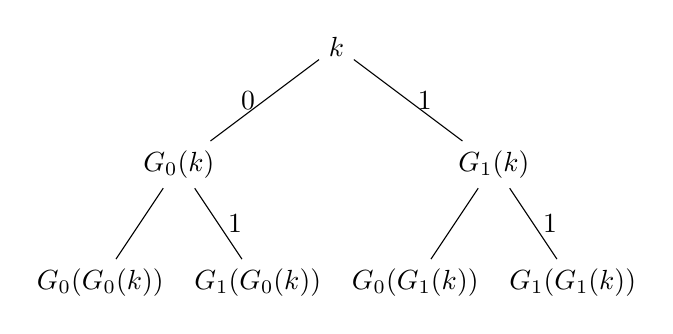
\begin{tikzpicture}[level distance=1.5cm,
  level 1/.style={sibling distance=4cm},
  level 2/.style={sibling distance=2cm}]
  \node {$k$}
    child {node {$G_0(k)$}
      child {node {$G_0(G_0(k))$}}
      child {node {$G_1(G_0(k))$} edge from parent node[right] {1}}
      edge from parent node[left] {0}
    }
    child {node {$G_1(k)$}
      child {node {$G_0(G_1(k))$}}
      child {node {$G_1(G_1(k))$} edge from parent node[right] {1}}
      edge from parent node[right] {1}
    };
\end{tikzpicture}
\end{center}
In general:\\
$$ F_k(x_1x_2...x_n) = G_{x_n}(G_{x_{n-1}}(...G_{x_1}(k)...)) $$
\end{defn}
\begin{thm}
    If $G$ is a secure PRG, then the GGM construction $F$ is a secure PRF. $\mathcal{F} = \{ f_k \}$ is a PRF.
\end{thm}
The proof relies on a hybrid argument and the following lemmas.

\begin{itemize}
    \item \textbf{Lemma 1}: If $G: \{0,1\}^n \to \{0,1\}^{2n}$ is a PRG, then for any polynomial $t(\lambda)$, the following two ensembles are computationally indistinguishable:
    $$ \{ (G(k_1), ..., G(k_t)) \} \approx_c \{ (U_{2n}, ..., U_{2n}) \}$$
    $$ k_1, ... , k_t \leftarrow U_n $$
    Next, given $F'_k \colon \{0,1\}^{n-1} \to \{0,1\}^n$ a PRF, then define:
    $$ F_k(x,y) = G_x(F'_{k}(y)) \text{ with } x \in \{0,1\}, y \in \{0,1\}^{n-1} $$
    \item \textbf{Lemma 2}: If $F'_k$ is a secure PRF, then $F_k$ is also a secure PRF.
\end{itemize}
Recall the GGM (Goldreich-Goldwasser-Micali) construction: 
$$ G:\{0,1\}^{\lambda}\rightarrow\{0,1\}^{2\lambda} $$ 
$$ G(k)=(G_{0}(k),G_{1}(k)) $$ 

We build $\mathcal{F}=\{F_{k}:\{0,1\}^{n(\lambda)}\rightarrow\{0,1\}^{\lambda}\}$ with $k \in \{0,1\}^{\lambda}$ such that 
$$ F_{k}(x)=G_{x_{n}}(G_{x_{n-1}}(...G_{x_{1}}(k)...)) $$ 
where $x = x_1x_2...x_n \in \{0,1\}^n$.

\subsection*{Proof of Security (by Induction)}

For the proof, let $n(\lambda) = \poly(\lambda)$. We use induction on $n$. 

Let $F_{k}^{'}:\{0,1\}^{n-1}\rightarrow\{0,1\}^{\lambda}$ be the GGM construction for inputs of length $n-1$. 
We can write $F_k$ for $n$-bit inputs as:
$$ F_{k}(x,y)=G_{x}(F_{k}^{'}(y)) $$ 
where $x\in\{0,1\}$ and $y\in\{0,1\}^{n-1}$. 

\begin{lem} 
If $\{F_{k}^{'}\}$ (GGM on $n-1$ inputs) is a PRF, then $\{F_k\}$ (GGM on $n$ inputs) is also a PRF family. 
\end{lem}

We can use this lemma to prove the security of GGM by induction. 

\subsubsection*{Base Case ($n=1$)} 
For $n=1$, the GGM construction is: 
$$ F_{k}(x)=G_{x}(k), \quad x \in \{0,1\} $$ 
This is:
$$ F_k(x) = \begin{cases} G_0(k) & \text{if } x=0 \\ G_1(k) & \text{if } x=1 \end{cases} $$ 
This is a PRF because $G$ is a PRG, so $(G_{0}(k),G_{1}(k))\approx_{c}U_{2\lambda}$. An adversary querying $F_k(0)$ and $F_k(1)$ just gets the output of the PRG, which is indistinguishable from two random $\lambda$-bit strings $R(0)$ and $R(1)$.

\subsubsection*{Inductive Step}
Assume $\{F_{k}^{'}\}$ (GGM on $n-1$ inputs) is a PRF. We want to prove $\{F_k\}$ (GGM on $n$ inputs) is a PRF. This is exactly what the Lemma states. 

\begin{proof}[Proof (of Lemma)] 
We use a hybrid argument. Let $\mathcal{A}$ be a PPT adversary.

\begin{itemize}
    \item \textbf{HYB 0}: The real world. 
    $$ z = F_{k}(x,y) = G_{x}(F_{k}^{'}(y)) $$ 
    where $k \leftarrow U_{\lambda}$. 
    
    \item \textbf{HYB 1}: 
    $$ z = G_{x}(R^{'}(y)) $$ 
    where $R^{'}: \leftarrow \mathcal{R}(\lambda,n-1 \rightarrow \lambda)$ is a truly random function from.
    
    \item \textbf{HYB 2}: The ideal world. 
    $$ z = R(x,y) $$ 
    where $R: \leftarrow \mathcal{R}(\lambda,n \rightarrow \lambda)$ is a truly random function.
\end{itemize}

\paragraph{Step 1: $HYB_0 \approx_c HYB_1$} 
We show $HYB_{0}(\lambda)\approx_{c}HYB_{1}(\lambda)$ by reduction. 
Assume a PPT $\mathcal{A}_{01}$ distinguishes $HYB_0$ and $HYB_1$ with non-negligible probability. 
We build a reduction $\mathcal{A}_{prf}$ that breaks the PRF security of $\{F_{k}^{'}\}$. 
\begin{center}
    \includegraphics[scale=0.4]{img/Comp_sec/Aprf.png}
\end{center}
If z = $F_{k}^{'}(y)$, then $G_{x}(z)$ is identical to what $\mathcal{A}_{prf}$ receives in $HYB_0$. On the other hand, if z = $R^{'}(y)$, then $G_{x}(z)$ is identical to what $\mathcal{A}_{prf}$ receives in $HYB_1$.\\
\paragraph{Step 2: $HYB_1 \approx_c HYB_2$} 
Here, we use the property that $G$ is a PRG. 

\begin{lem}[PRG Expansion]
If $G:\{0,1\}^{\lambda}\rightarrow\{0,1\}^{2\lambda}$ is a PRG, then for any $t = \poly(\lambda)$: 
$$ (G(k_{1}),\dots,G(k_{t})) \approx_{c} (U_{2\lambda},\dots,U_{2\lambda}) \equiv U_{2\lambda \cdot t} $$ 
where $k_{1},\dots,k_{t} \leftarrow U_{\lambda}$ are chosen independently. 
\end{lem}

Now, assume a PPT $\mathcal{A}_{12}$ distinguishes $HYB_1$ and $HYB_2$. We build a PPT $\mathcal{A}_{prg}$:breaking the above claim.
\begin{center}
    \includegraphics[scale=0.4]{img/Comp_sec/claim.png}
\end{center}
Let $t(\lambda) = q(\lambda)$ - the number of queries made by $\mathcal{A}_{12}$. Each of $z_i \in \{0,1\}^{2\lambda}$ and we can think of it as:
$$ z_i = (z_{i}^0, z_{i}^1) $$
With each corresponding to $\lambda$ bits.\\

In the above reduction, $i(y)$ is the index of the sample $z_i$ that was used when $\mathcal{A}_{12}$ asked already for x,y. If it never asked use the next available $z_i$.

\end{proof}

In the next few lectures, we'll see PRFs are enough to do practical symmetric crypto: 
\begin{itemize}
    \item CPA-Secure SKE (Symmetric Key Encryption) for messages of variable length (VIL). 
    \item MACs (Message Authentication Codes) for messages of VIL. 
    \item Non-malleable SKE (a.k.a. CCA-Secure SKE), which is equivalent to combining message privacy and message authentication. 
\end{itemize}

It will be important that our PRF $F$ is a \textbf{PRP (Pseudorandom Permutation)}, namely it is an efficient, length-preserving permutation for a given key. 
In practice, we call it a \textbf{BLOCKCIPHER}. We will show that $PRPs \approx PRFs$. 
This will also explain the real-world design of some blockciphers (e.g., DES, AES). 

\section*{CPA-Secure SKE for Variable Length Messages}
Let's start with encryption (CPA-security). 
Recall the CPA indistinguishability game ($\game^{CPA}$): 
The adversary $\mathcal{A}$ submits two messages $m_0, m_1$ of the same length ($|m_0| = |m_1|$) to a challenger. The challenger picks $k \leftarrow \mathcal{K}$, computes $c \leftarrow \enc(k, m_b)$ for a random bit $b$, and sends $c$ to $\mathcal{A}$. $\mathcal{A}$ wins if it guesses $b$.
We need this to work for messages of any polynomial length (VIL). 

\subsection*{Mode of Operation} 
A mode of operation is a standardized way to encrypt messages $m = (m_1, \dots, m_d)$, where $m_i \in \{0,1\}^n$, using a PRF $\mathcal{F} = \{F_k: \{0,1\}^n \rightarrow \{0,1\}^n\}$. 

\begin{rem}
We can't just use $c = (F_k(m_1), \dots, F_k(m_d))$. This is Electronic Codebook (ECB) mode, and it's not secure (it leaks equalities between blocks). This is true even if $F$ is a PRP. 
\end{rem}

\subsubsection*{CBC (Cipher Block Chaining) Mode} 
\begin{itemize}
    \item $c_0 = IV \in U_n$ (Initialization Vector) 
    \item $c_i = F_k(c_{i-1} \oplus m_i)$ for $i=1, \dots, d$ 
    \item Output: $c = (c_0, c_1, \dots, c_d)$ 
\end{itemize}
\begin{center}
    \includegraphics[scale=0.4]{img/Symmetric/CBC.png}
\end{center}
Decryption requires $F_k^{-1}$, so $F$ must be a PRP. Encryption is sequential. 
\begin{thm}
If $F$ is a PRP, then CBC-Mode is CPA-secure for VIL. 
\end{thm}

\subsubsection*{OFB (Output Feedback) Mode} 
\begin{itemize}
    \item $c_0 = r \in U_n$ 
    \item $k_0 = r$
    \item $k_i = F_k(k_{i-1})$ for $i=1, \dots, d$ 
    \item $c_i = k_i \oplus m_i$ for $i=1, \dots, d$ 
    \item Output: $c = (c_0, c_1, \dots, c_d)$
\end{itemize}
\begin{center}
    \includegraphics[scale=0.4]{img/Symmetric/OFB.png}
\end{center}

\subsubsection*{CTR (Counter) Mode} 
\begin{itemize}
    \item $c_0 = r \in U_n$ (where $r$ is a counter) 
    \item $c_i = F_k(r+i-1) \oplus m_i$ for $i=1, \dots, d$ 
    \item Output: $c = (c_0, c_1, \dots, c_d)$
    \item Note: "$+$" can be modulo $2^n$ arithmetic. 
\end{itemize}
\begin{center}
    \includegraphics[scale=0.4]{img/Symmetric/CTR.png}
\end{center}

\begin{thm}
Assuming $F$ is a PRF, CTR mode is a CPA-secure SKE for VIL. 
\end{thm}
\begin{proof}
We use a hybrid argument.
Let $G(\lambda, b) \equiv \game_{\Pi}^{cpa}(\lambda, b)$ be the CPA game where $\Pi$ is CTR mode using $\mathcal{F}$. We want to show $G(\lambda, 0) \approx_c G(\lambda, 1)$. 
Recall that in $G(\lambda,0)$:\\
Upon input an encryption query $m = (m_1, \dots, m_d)$, we return $c = (c_1, \dots, c_d)$ such that $c_0 = r \in U_n$ and $c_i = F_k(r+i-1) \oplus m_i$.\\
For the challenge $m_b^* = (m_{b,1}^*, \dots, m_{b,d^*}^*) (d^* \in \N is the dimension)$, we return $c^* = (c_0^*, \dots, c_{d^*}^*)$ such that $c_0^* = r^* \in U_n$ and $c_i^* = F_k(r^*+i-1) \oplus m_{b,i}^*$.\\
\begin{itemize}
    \item \textbf{Game $G(\lambda, b)$}: Real game.
    \begin{itemize}
        \item Encryption query $m=(m_1, \dots, m_d)$: return $c=(c_0, \dots, c_d)$ where $c_0 = r \in U_n$ and $c_i = F_k(r+i-1) \oplus m_i$. 
        \item Challenge query $m_b^*$: return $c^*=(c_0^*, \dots, c_{d^*}^*)$ where $c_0^* = r^* \in U_n$ and $c_i^* = F_k(r^*+i-1) \oplus m_{b,i}^*$. 
    \end{itemize}
    \item \textbf{Hybrid $H_1(\lambda, b)$}: Same as $G(\lambda, b)$, but replace $F_k(\cdot)$ with a truly random function $R(\cdot)$. 
    \item \textbf{Hybrid $H_2(\lambda)$}: The challenge ciphertext $c^*$ is uniform and independent of $b$. (i.e., $c_0^* = r^*$ and $c_i^* = u_i \oplus m_{b,i}^*$ where $u_i$ are fresh uniform strings. This is equivalent to $c^*$ being $c_0^*$ and $d^*$ fresh uniform strings, which is independent of $b$.)
\end{itemize}

\begin{lem}
$G(\lambda, b) \approx_c H_1(\lambda, b)$ for all $b \in \{0,1\}$.
\end{lem}
\begin{proof}
Standard reduction. Fix $b$. Assume a PPT $\mathcal{A}$ distinguishes $G(\lambda, b)$ and $H_1(\lambda, b)$. We build a PPT adversary $\mathcal{A}_prf$ against the PRF $F$.
\begin{center}
    \includegraphics[scale=0.4]{img/Symmetric/lem1proof.png}
\end{center}
\end{proof}

\begin{lem}
$H_1(\lambda, b) \approx_c H_2(\lambda)$, as long as the number of encryption queries $q(\lambda) = \poly(\lambda)$. 
\end{lem}
\begin{proof}
In $H_1(\lambda, b)$, the challenge ciphertext is created using the values $R(r^*), R(r^*+1), \dots, R(r^*+d^*-1)$. An encryption query $j$ uses values $R(r_j), R(r_j+1), \dots, R(r_j+d_j-1)$. 

Let \textbf{BAD} be the event that any counter value used for the challenge overlaps with any counter value used for any encryption query. 
$$ \text{BAD} = \exists j, i, i' \text{ s.t. } r^*+i' = r_j+i $$ 
($i' \in [0, d^*-1]$, $i \in [0, d_j-1]$)

Conditioned on $\neg \text{BAD}$, all values $r^*+i'$ are "fresh" inputs to the random function $R$. This means all outputs $R(r^*+i')$ are independent and uniformly random. In this case, $c_i^* = R(r^*+i-1) \oplus m_{b,i}^*$ is a one-time pad encryption, and the ciphertext $c^*$ is uniform and independent of $b$. This is exactly $H_2(\lambda)$. 

By the properties of statistical distance:
$$ SD(H_1(\lambda, b); H_2(\lambda)) \le \Pr[\text{BAD}] $$ 

We just need to bound $\Pr[\text{BAD}]$. Let $q = q(\lambda)$ be the number of queries.
Let $\text{BAD}_j$ be the event that the challenge overlaps with query $j$. 
$\Pr[\text{BAD}] = \Pr[\cup_{j=1}^q \text{BAD}_j] \le \sum_{j=1}^q \Pr[\text{BAD}_j]$ (by Union Bound). 

Let's bound $\Pr[\text{BAD}_j]$. WLOG, assume all message lengths are at most $q$. 
Overlap $\text{BAD}_j$ occurs if $\{r^*, \dots, r^*+q-1\}$ overlaps with $\{r_j, \dots, r_j+q-1\}$. 
$r^*$ and $r_j$ are chosen uniformly from $\{0, \dots, 2^n-1\}$.
Overlap happens if $r_j \in [r^*-q+1, r^*+q-1]$. 
The size of this interval is $(r^*+q-1) - (r^*-q+1) + 1 = 2q-1$.
So, $\Pr[\text{BAD}_j] = \frac{2q-1}{2^n}$. 

$$ \Pr[\text{BAD}] \le \sum_{j=1}^q \frac{2q-1}{2^n} = q \cdot \frac{2q-1}{2^n} \le \frac{2q^2}{2^n} = \negl(\lambda) $$ 
Since $q = \poly(\lambda)$ and $n$ (the block size) is related to $\lambda$ (e.g., $n=\lambda$), $2^n$ is exponential in $\lambda$.
\end{proof}

\textbf{Conclusion}:
$G(\lambda, 0) \approx_c H_1(\lambda, 0) \approx_c H_2(\lambda) \approx_c H_1(\lambda, 1) \approx_c G(\lambda, 1)$. 
The advantages $G(\lambda, 0) \approx_c H_1(\lambda, 0)$ and $H_1(\lambda, 1) \approx_c G(\lambda, 1)$ are negligible by Lemma 1.
The advantages $H_1(\lambda, 0) \approx_c H_2(\lambda)$ and $H_2(\lambda) \approx_c H_1(\lambda, 1)$ are negligible by Lemma 2.
Thus, $G(\lambda, 0) \approx_c G(\lambda, 1)$ by the triangle inequality, and CTR mode is CPA-secure. 
\end{proof}

\subsection{Message Authentication Codes (MACs)}

We now switch to the problem of message authentication. 
We need a security guarantee that it is computationally hard to forge a message/tag pair $(m^*, \tau^*)$ such that $\text{Vrfy}(k, m^*) = \text{accept}$ (or $\text{Tag}(k, m^*) = \tau^*$) without knowing the secret key $k$. 

\begin{defn}[UF-CMA]
We say a MAC scheme $\Pi = (\text{Gen}, \text{Tag}, \text{Vrfy})$ is \textbf{Unforgeable Under a Chosen-Message Attack (UF-CMA)} if for all PPT adversaries $\mathcal{A}$, $\Pr[\game_{\Pi, \mathcal{A}}^{ufcma}(\lambda) = 1] \le \negl(\lambda)$. 

The game $\game_{\Pi, \mathcal{A}}^{ufcma}(\lambda)$ proceeds as follows: 
\begin{enumerate}
    \item $k \leftarrow \text{Gen}(\lambda)$ 
    \item $\mathcal{A}$ gets oracle access to $\text{Tag}(k, \cdot)$. $\mathcal{A}$ makes queries $m_1, \dots, m_q$ and receives $\tau_i = \text{Tag}(k, m_i)$. 
    \item $\mathcal{A}$ outputs a pair $(m^*, \tau^*)$. 
    \item $\mathcal{A}$ wins if $\text{Vrfy}(k, m^*) = \text{accept}$ (i.e., $\text{Tag}(k, m^*) = \tau^*$) AND $m^* \notin \{m_1, \dots, m_q\}$. 
\end{enumerate}
\end{defn}

\begin{thm}
If $\mathcal{F} = \{F_k\}$ is a PRF, then the MAC scheme $\text{Tag}(k, m) = F_k(m)$ is UF-CMA for fixed-length messages. 
\end{thm}
\end{document}